Per il training del modello si è utilizzato un dataset pubblico rilasciato da Google\footnote{Open Image V6, \url{https://storage.googleapis.com/openimages/web/index.html?v6}} contenente 10 mila immagini di visi umani, dove ogni foto conteneva da uno a più visi umani.

Oltre alle immagini il dataset conteneva un utile file \textit{Excel} che indicava le coordinate della posizione degli occhi delle persone all'interno dell'immagine.

Prima dell'addestramento della rete era però necessario convertire questi dati di input in file \textit{*.xml} in modo tale da poterli poi usare per generare i \textbf{TFRecord}, utili per TensorFlow. Per questo motivo è stato implementato uno script \textit{Java} in grado di creare un file \textit{.xml} per ogni foto del dataset estraendo le informazioni dal file \textit{Excel}. Le informazioni più importanti per il nostro progetto che sono state estratte sono: i dati geografici delle posizioni degli occhi (x e y, sia min che max) e il nome del'oggetto da riconoscere.

Inoltre, per la corretta generazione dei \textbf{TFRecord}, si è reso necessario compilare il file \textit{labelmap.pbtxt} con al suo interno i nomi e gli id dei nostri oggetti da riconoscere: nel nostro caso un solo item di id pari a 1 e con nome "Human eye".

\begin{figure}[htbp]
    \centering
    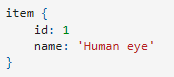
\includegraphics[scale=1]{ReteNeurale/EyeDetection/Dataset/Images/eyelabelmap_item.png}
    \caption{Eye Detection labelmap.pbtxt}
    \label{fig:eyelabelmap}
\end{figure}